\section{Punto de Vista de la Realización de Objetivos}

El punto de vista de la realización de objetivos permite a un diseñador modelar el refinamiento de los objetivos (de alto nivel) en objetivos más tangibles, y el refinamiento de los objetivos tangibles en requisitos o restricciones que describen las propiedades que se necesitan para realizar los objetivos. El refinamiento de los objetivos en subobjetivos se modela utilizando la relación de agregación. El refinamiento de los objetivos en requisitos se modela utilizando la relación de realización.
Además, se pueden modelar los principios que guían el refinamiento de las metas en requisitos.

\subsection{Modelo de la Realización de Objetivos}
\begin{figure}[h!]
	\centering
	\includegraphics[width=1.0\linewidth]{imgs/modelo/RealObjetivos.pdf}
	\caption{Modelo Realización de Objetivos}
\end{figure}

La motivación de una organización o persona para lograr ciertos resultados está representada por las metas, los principios, los requisitos y las limitaciones. Las metas representan que un interesado quiere lograr un determinado resultado; por ejemplo, "Aumentar la satisfacción del cliente en un 10\%". Los resultados finales obtenidos por las capacidades que realizan estas metas son los resultados.

Un objetivo representa una declaración de intenciones de alto nivel, una dirección o un estado final deseado para una organización y sus partes interesadas.

\newpage

\subsection{Caso de la Realización de Objetivos}
\begin{figure}[h!]
	\centering
	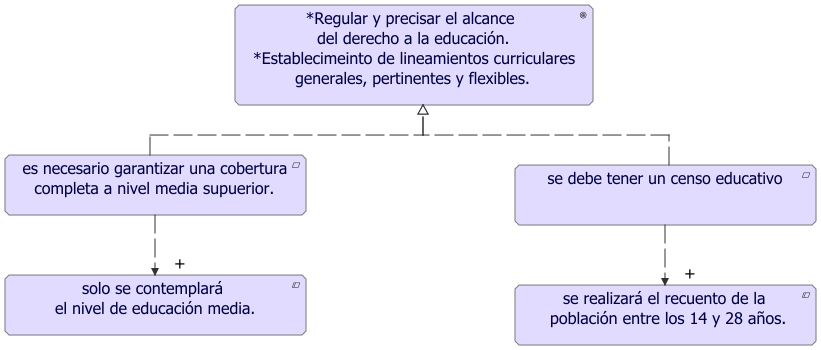
\includegraphics[width=1.0\linewidth]{imgs/motivacion/realizacionObj/realizacion.pdf}
	\caption{Caso Realización de Objetivos}
\end{figure}

Los requerimientos necesarios para regular y precisar el alcance del derecho a la educación, así como para dar alcance al objetivo de establecer los lineamientos curriculares, generales, pertinentes y flexibles radican en garantizar una cobertura completa en la educación media superior del país, que permita abrir una brecha para la implantación de esta ofertas educativas con aras de que logren mantenerse y adquirir una mayor demanda a través de las regulaciones del MEN para dar alcance al derecho de la educación a toda la comunidad. Igualmente, otro requerimiento indispensable para la consecución de estos objetivos planteados, es la realización de un censo educativo que proporcione un conocimiento certero sobre las características de la población a la cual está dirigida esta política inclusiva de educación y que además, provea de información vitalicia para la construcción y/o adecuación de las ofertas educativas de lineamientos curriculares generales, flexibles, pertinentes y flexibles. \\ \\
No obstante, una limitación en el requerimiento dispuesto para la garantía de una cobertura completa a nivel media superior es que, solo se contemplará la identificación vocacional en la transición de un nivel de educación media a superior, postergando la identificación vocacional a través de la gamificación en la transición de educación básica a educación media. A causa de este limitante, el censo educativo, aunque se realizará de forma general, en su etapa posterior del proceso, solo se hará énfasis en el recuento de la población entre los 14 y 28 años.